% !TEX root = ../main.tex
% chktex-file 17
% chktex-file 21
\section{Optimizing Training}%
\label{sec:params}

Now follows an overview of approaches to speed up the training process.
We will discuss four approaches:
\begin{enumerate}
	\item A general purpose method that combines subsampling with bootstrapping.
	\item An iterative method to select the optimal subsample size during gradient descent.
	\item Improving the quality of subsampling for logistic regression by weighing the samples.
	\item Speeding up the training of SVMs via \(k\)-means clustering.
\end{enumerate}

\subsection{Bag of Little Bootstraps}%
\label{sec:params:blb}

The first approach we will discuss is called \textit{Bag of Little Bootstraps}~(BLB)~\cite{Kleiner2011}.
It combines subsampling with bootstrapping and is particularly well suited for parallelized implementations.

In the context of Big Data training typically cannot be performed on the entire dataset.
A na{\"\i}ve way to solve this problem is to simply train on a random \(b\) out of \(n\) subsample of the data \(\Dtrain = \{X_1, \dots, X_n\}\).
This approach is highly sensitive to noise in the training dataset, especially if \(b \ll n\).
To overcome this problem bootstrapping can be used.
The regular \(n\) out of \(n\) bootstrapping technique for variance reduction is not suitable for big datasets because it uses \(63\%\) of the training data on average.
However the \textit{\(b\) out of \(n\) bootstrapping} (BOFN) approach can in principle be applied.
It uses \(s\) samples \(\{\check{X}^{(i)} = (\check{X}_1^{(i)}, \dots, \check{X}_b^{(i)})\, |\, 1 \leq i \leq s\}\) of \(b\) datapoints each.
Since this approach independently learns \(s\) hypotheses \(h_i\) on small datasets \(\check{X}^{(i)}\), their parameterizations \(\theta_i\) tend to have large confidence intervals.
Because of that, the quality of the combined hypothesis is strongly dependent on \(b\).
BLB reduces this dependence.

\subsubsection{Intuition}%
\label{sec:params:blb:intuition}

\begin{figure}
	\centering
	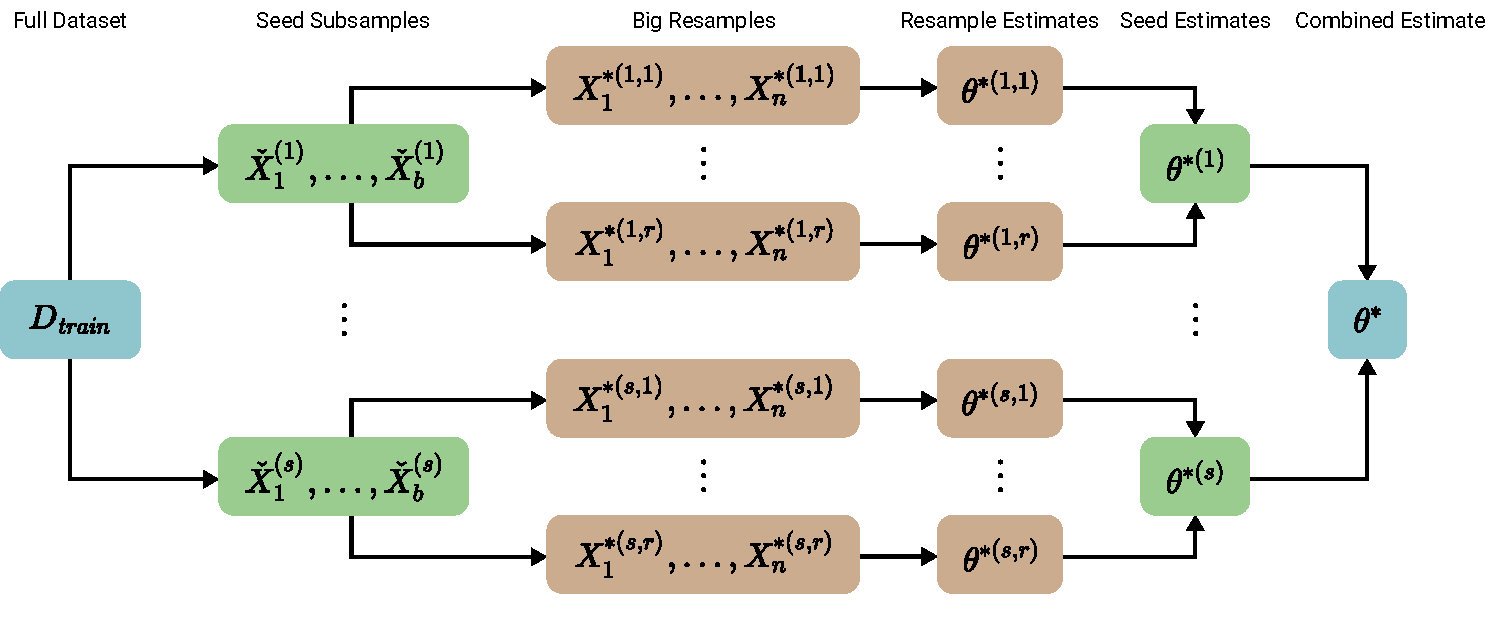
\includegraphics[width=\linewidth]{gfx/blb/overview.pdf}
	\caption{Overview of the steps of BLB.}\label{fig:blb:overview}
\end{figure}
BLB is a simple extension of BOFN that is consistently more robust regarding the choice \(b\) across datasets.
The basic idea is to add another sampling step.
BLB uses each subsample \(\check{X}^{(i)}\) as a seed for \(n\) out of \(b\) sampling.
This yields bigger resamples \(\{X^{*(i, k)} = (X_1^{*(i, k)}, \dots, X_n^{*(i, k)})\, |\, 1 \leq i \leq s, 1 \leq k \leq r\}\) that each contain at most \(b\) different elements.
Training is then run on the resamples \(X^*\) instead of the small seed samples \(\check{X}\).
The learned hypothesis parameterizations are finally combined to a single hypothesis parameterization \(\theta^*\) via a model specific combination function, e.~g.\@ by simply taking the average.
Figure~\ref{fig:blb:overview} illustrates those steps.

Even though BLB trains classifiers on resamples of size \(n\) its time and space complexity effectively still depends on \(b\), not \(n\).
This is because each resample \(X^*\) only contains at most \(b\) different elements which means that it can be efficiently represented by a list of \(b\) multiplicity counts \((c_1, \dots, c_b) \in \mathbb{N}^b\), i.~e.\@ \(\mathit{space} = \mathcal{O}(b \log n)\).
Training on such a dataset is equivalent to training on a dataset of size \(b\) with weights \(w_i = \frac{c_i}{n}\).
Since most commonly used classifiers support weighted samples, BLB is widely applicable.

\subsubsection{Evaluation}%
\label{sec:params:blb:eval}

To show the advantages of BLB for classification it was evaluated with logistic regression.
Figure~\ref{fig:blb:eval:single} shows that BLB converges on a solution much faster than the regular \(n\) out of \(n\) bootstrapping (BOOT) with comparable results.
It also shows that BLB is less sensitive to the choice of \(b\) than BOFN.\
BLB reached good results with \(b \geq n^{0.6}\) whereas BOFN required at least \(b \geq n^{0.7}\).

While BLB already outperforms BOOT without parallelism, as training is overproportionally faster on small samples, its scalability becomes more apparent when parallelized.
Figure~\ref{fig:blb:eval:parallel} shows that BLB significantly outperforms BOOT on a Spark cluster with 10 workers.
This is due to the fact that each BLB sample can be held in memory by its corresponding worker node.
The much larger BOOT samples, on the other hand, require disk reads for large datasets.
\begin{figure}
	\begin{subfigure}[t]{0.67\textwidth}
		\centering
		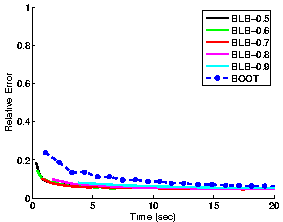
\includegraphics[width=0.49\linewidth]{gfx/blb/time1.pdf}
		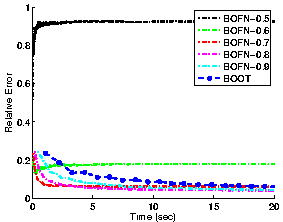
\includegraphics[width=0.49\linewidth]{gfx/blb/time2.pdf}
		\caption{
			Single-threaded results on a subset of the data.
			\(b = n^\gamma\) for multiple values of \(\gamma \in [0.5, 1]\) and \(r = 100\) is used.
			\(s\) is not fixed and grows over time.
		}\label{fig:blb:eval:single}
	\end{subfigure}
	\begin{subfigure}[t]{0.32\textwidth}
		\centering
		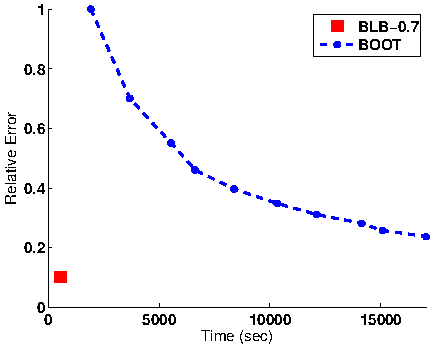
\includegraphics[width=\linewidth]{gfx/blb/parallel.pdf}
		\caption{
			Parallelized results on the entire dataset.
			\(b = n^{0.7}\), \(s = 5\) and \(r = 50\) is used for BLB.\
			For BOOT \(s\) grows over time.
		}\label{fig:blb:eval:parallel}
	\end{subfigure}
	\caption{
		Comparison of BLB and BOFN with BOOT using logistic regression.
		Shows the error on the moving average of all sample hypotheses that are computed within a given time.
	}\label{fig:blb:eval}
\end{figure}

\subsection{Subsample Size Selection for Gradient Descent}%
\label{sec:params:samplesize}

Next we will discuss an optimization technique for \textit{stochastic gradient descent} (SGD).
The size of the subsample \(\mathcal{S}\) that is considered in a single gradient descent step heavily influences the optimizer's behavior:
\begin{itemize}
	\item In the stochastic approximation regime small samples, typically \(|\mathcal{S}| = 1\), are used. This causes fast but noisy steps.
	\item In the batch regime large samples are used, typically \(|\mathcal{S}| = N\) with \(N := |\Dtrain|\). Steps are expensive to compute but more reliable.
\end{itemize}
Both extremes are usually not suitable for Big Data applications.
Very small samples cannot be parallelized well, making them a bad fit for the compute clusters that are typically available nowadays.
The gradients for very big samples however are often too slow to compute.
\(|\mathcal{S}|\) should ideally lie somewhere in between.

\subsubsection{Size Selection Method}%
\label{sec:params:samplesize:method}

\citet{Byrd2012} describe an iterative algorithm that dynamically increases the size of \(\mathcal{S}\) as long as this promises to significantly reduce the gradient noise.
Let \(\mathcal{S} \subseteq \{1, \dots, N\}\) describe a random subsample of \(\Dtrain = \{(x_i, y_i)\, |\, 1 \leq i \leq N\}\).
SGD will take a step in the descent direction \(d = -\nabla J_{\mathcal{S}}(w)\) where \(J_{\mathcal{S}}(w) := \frac{1}{|\mathcal{S}|} \sum_{i \in \mathcal{S}} \ell(h_{w}(x_i), y_i)\) is the differentiable average loss on \(\mathcal{S}\) given the current configuration \(w\).
Let \(J(w)\) be the average loss on the entire dataset.
\(J(w)\) is the objective function we want to minimize.
Our goal is to trade off \(|\mathcal{S}|\) s.~t.\@ it is as small as possible and \(\nabla J_{\mathcal{S}}\) still \textit{tends to agree} with the objective gradient \(\nabla J(w)\), or more formally
\begin{align}
	\|\nabla J_{\mathcal{S}}(w) - \nabla J(w) \|_2 \leq \theta \|\nabla J_{\mathcal{S}}(w)\|_2, \theta \in [0, 1)\label{eq:samplesize:cond} % chktex 9
\end{align}
A value of \(\theta = 0\) means that \(\nabla J_{\mathcal{S}}(w)\) always has to be equal to \(\nabla J(w)\),
whereas \(\theta = 1\) would allow steps that directy oppose \(\nabla J(w)\).
Since it is infeasible to compute \(\nabla J(w)\), condition (\ref{eq:samplesize:cond}) can however not be checked directly.
We will instead resort to an estimate and check whether the condition is satisfied in expectation:
\begin{align}
	\underbrace{\mathbb{E}_{\mathcal{S}}[\|\nabla J_{\mathcal{S}}(w) - \nabla J(w) \|_2^2]}_{= \|\mathrm{Var}_{\mathcal{S}}(\nabla J_{\mathcal{S}}(w))\|_1} \leq \theta^2 \|\nabla J_{\mathcal{S}}(w)\|_2^2\label{eq:samplesize:exp}
\end{align}
Computing \(\mathrm{Var}_{\mathcal{S}}(\nabla J_{\mathcal{S}}(w))\) directly is also infeasible because it would require considering all samples of a certain size.
Given a sample \(\mathcal{S}\), the variance of all samples of that size can instead be approximated using
\begin{align}
	\|\mathrm{Var}_{\mathcal{S}}(\nabla J_{\mathcal{S}}(w))\|_1 \approx \frac{1}{|\mathcal{S}| (|\mathcal{S}| - 1)} \sum_{i \in \mathcal{S}} \|\nabla \ell(h_w(x_i), y_i) - \nabla J_{\mathcal{S}}(w)\|_2^2\label{eq:samplesize:approx}
\end{align}
Using (\ref{eq:samplesize:approx}) we can now estimate (\ref{eq:samplesize:exp}) which in turn estimates (\ref{eq:samplesize:cond}).
If the condition is not satisfied, i.~e.\@ the sample gradient is likely to deviate from the objective gradient, we will have to use a larger sample \(\widehat{\mathcal{S}}\).
In principle we could simply increase the sample size by a constant amount repeatedly and recheck (\ref{eq:samplesize:exp}) but this is slow if \(|\mathcal{S}|\) is far off from satisfying the condition.
Instead we will adaptively choose \(|\widehat{\mathcal{S}}|\) s.~t.\@ it is expected to satisfy (\ref{eq:samplesize:exp}):
\begin{align}
	|\widehat{\mathcal{S}}| = \frac{|\mathcal{S}|\, \|\mathrm{Var}_{\mathcal{S}}(\nabla J_{\mathcal{S}}(w))\|_1}{\theta^2 \|\nabla J_{\mathcal{S}(w)}\|_2^2}\label{eq:samplesize:inc}
\end{align}
See \citet[Chapter 3]{Byrd2012} for a more detailed explanation of (\ref{eq:samplesize:approx}) and (\ref{eq:samplesize:inc}).
To incorporate the ideas described above into SGD (\ref{eq:samplesize:exp}) has to be checked after each gradient descent step.
If the check fails, the size of the following samples has to be increased according to (\ref{eq:samplesize:approx}).
Good values for the initial sample size and for \(\theta\) have to be found via hyperparameter optimization.

\subsubsection{Evaluation}%
\label{sec:params:samplesize:eval}

\begin{tikzpicture}
	\begin{axis}[
		xmin=0, xmax=8,
		ymin=0, ymax=0.14,
		xtick distance=1,
		ytick distance=0.02,
		y tick label style={/pgf/number format/.cd, fixed},
		xlabel={No.\@ of Accessed Data Points}
	]
		\addplot table [x=x, y=FG5, col sep=comma] {data/samplesize/performance.csv};
		\addplot table [x=x, y=FG100, col sep=comma] {data/samplesize/performance.csv};
		\addplot table [x=x, y=Dynamic, col sep=comma] {data/samplesize/performance.csv};
	\end{axis}
\end{tikzpicture}

\subsection{Subsampling for Logistic Regression}%
\label{sec:params:osmac}

Subsampling usually increases the mean squared error (MSE) of the resulting hypothesis compared to one that is trained on the full dataset.
OSMAC~\cite{Wang2017} is a method that improves upon na{\"\i}ve subsampling by weighing the samples.

\textit{TODO:\@ explain OSMAC}

\subsection{SVM-KM}%
\label{sec:params:svmkm}

To speed up the training of SVMs \citet{Almeida2000} proposed a simple method that reduces the dataset size via \(k\)-means clustering.
It can be described as a three-step procedure:
\begin{enumerate}
	\item Group the training samples \(\Dtrain\) into \(k\) clusters \(C_1, \dots, C_k\) with centers \(c_1, \dots, c_k\) where \(k\) should be determined via hyperparameter optimization.
	\item Check for each cluster \(C_i\) whether all associated datapoints belong to the same class, i.~e.\@ \(\exists\, z \in \{+1, -1\}: \forall (x, y) \in C_i: y = z\).
		If yes, all datapoints in \(C_i\) are removed from \(\Dtrain\) and replaced by \(c_i\).
		If not, they are kept in the dataset.
		The intuition behind this is that clusters with points from multiple classes might be near the decision boundary so they are kept to serve as potential support vectors.
	\item Finally standard SVM training is performed on the reduced training dataset.
\end{enumerate}

\subsubsection{Evaluation}%
\label{sec:params:svmkm:eval}

\textit{TODO}
